\chapter{Related Works}
\label{chap-related-works}
\begin{ChapAbstract}
In this chapter, introduce the volume organs segmentation problem, inspire from video object segmentation problem and is most related to our work. We also discuss the semi-supervised approaches which are widely used to solve medical image segmentation task and details about the state-of-the-art model that we utilized in our system in section \ref{sec:segmentation} and \ref{sec:semisup} 
Next, we introduce related works which have a same scenario and motivation to solve the interactive segmentation concept. We provide detailed discussions about the Interactive methods and Positional encoding technique which applied directly to our propose architecture in section \ref{sec:mask_propagate} and section \ref{sec:positional_encoding}).
\end{ChapAbstract}
% \section{Video-text retrieval}
\label{sec:video-text_ret}
Representation Learning (RL) aims to learn compact features of high-dimensonal data (e.g. image, video, audio or document), which has a range of applications in cross-modal context matching. Especially between visual and textual information, it learns to embed the vision and language information into the same latent space, where similarities of different modal features reflect the proximity of their original semantics. \\
The image-text matching task is related to various problems such as Image Captioning (\cite{vinyals2015show, xu2015show, anderson2018bottom}), Image-Text retrieval (\cite{radenovic2018fine, vo2019composing, revaud2019learning}) and Visual Question Answering (\cite{xu2016ask, goyal2017making, anderson2018bottom}), to name a few.
In other scenarios, when one static image cannot provide the full meaning of a concept, which needs the spatio-temporal information from a sequence of images as a video, the video-text matching takes place. 
In the area of video-text retrieval, more and more researchers are paying more attention to RL-based modeling.
Common methods (\cite{lin2014visual, yu2017end, mithun2018learning, miech2018learning, dong2019dual}) utilize popular pretrained word embedding models (Word2vec \cite{mikolov2013efficient}, Glove \cite{pennington2014glove}, etc.) along with sequential models (LSTM \cite{hochreiter1997long}, GRU \cite{cho2014learning}) to construct textual feature extractors. For visual modeling, while some works (\cite{zhang2018cross, miech2020end}) utilize Conv3D based backbones (C3D \cite{carreira2017quo}, S3D \cite{xie2018rethinking}), others use pretrained Conv2D networks to encode frame-level features, and aggregate these features into a video-level representation by a sequential model or pooling function, \cite{li2019w2vv++,ging2020coot}. 
\begin{figure}[t!]
    \centering
    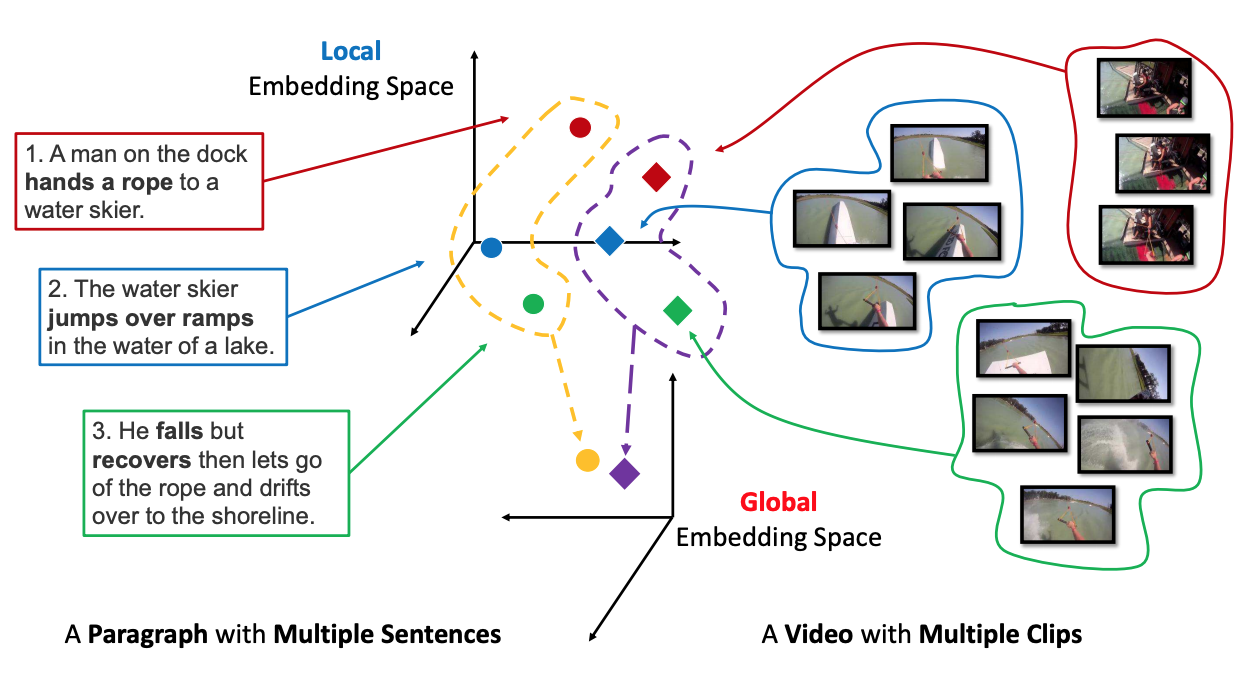
\includegraphics[width=0.9\textwidth]{images/long_vid-text.png}
    \caption{A conceptual diagram illustrates the process of modeling long-range input. The sentence/clip and paragraph/video pair is represented in local and global space respectively. \cite{zhang2018cross}}
    \label{fig:long_vidtext}
\end{figure}
Further, some works deal with long-range video-text relationship, in which video input is a set of consecutive clips, each displays a specific event and text data is a paragraph of multiple sentences describing those events in the respective order. 
Zhang et al. \cite{zhang2018cross} constructs a hierarchical architecture with different levels: video/paragraph, clip/sentence, frame/word to capture the whole temporal context, and apply losses that enforces the interaction between and within different hierarchy levels (shown in Figure \ref{fig:long_vidtext}). Ging, Simon, et al. \cite{ging2020coot} utilizes the objective function from Zhang et al. \cite{zhang2018cross} and proposes a new transformer-based architecture along with a trainable aggregation function to learn better representation. In this work, we adopt these modules to build a RL-based retrieval module, which is also used as a baseline for further improvements.\\
In some cases when the retrieval targets based on some specific details, and the video may contain abundant relations, those aformentioned methods could pay less attention to those important relations, which leads to worse performance. The RL-based architectures now need to enhance those semantic representations when modeling. Feng, Zerun, et al \cite{feng2020exploiting} address the issue by generating region features with semantic relations for frame-level embeddings. Chen, Shizhe, et al \cite{chen2020fine} proposes a hierarchy of three-level semantic matching: event level (based on whole input sentence), actions and entities denoted by verbs and noun phrases respectively. Taking inspiration from these approaches, we propose a relation module to extract semantic relationships between targets and neighboring objects.


% \section{Natural language-based vehicle retrieval}
\label{sec:ai_city}
\begin{figure}[!ht]
    \centering
    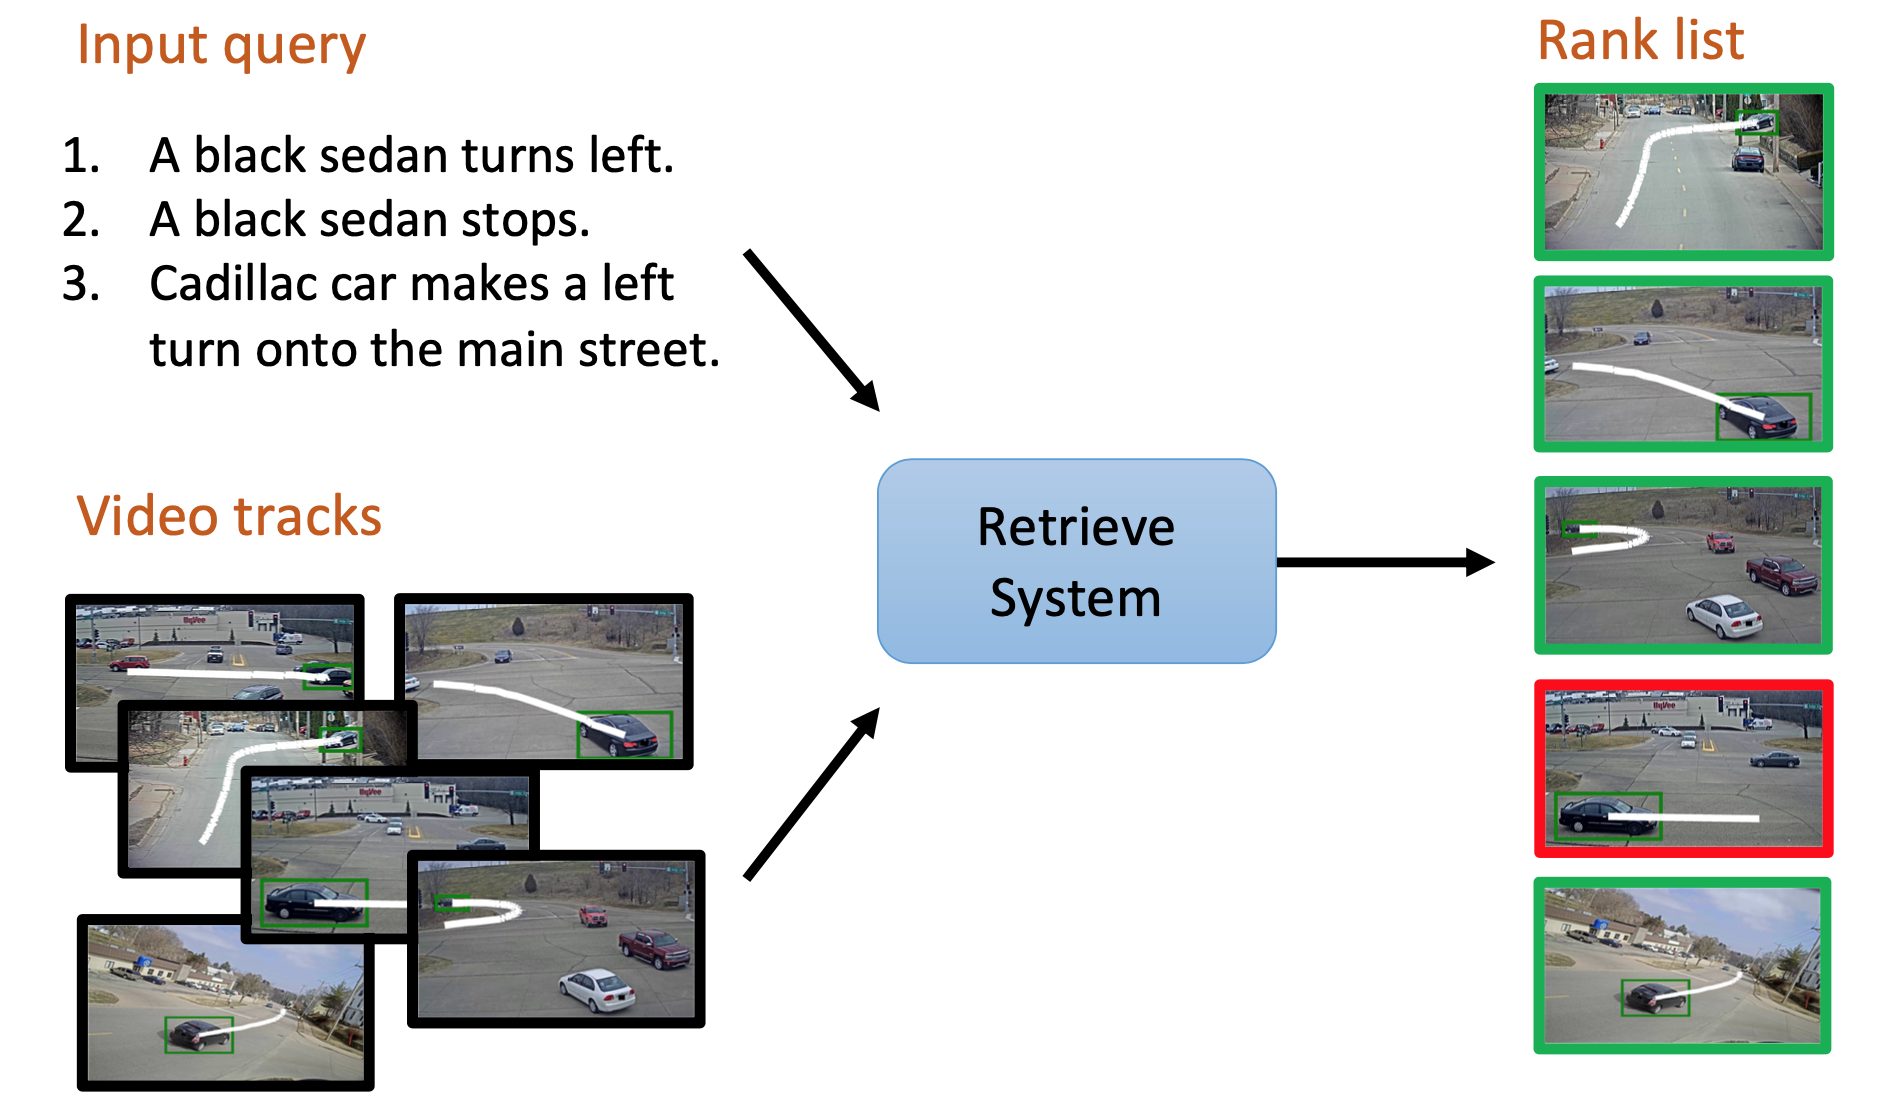
\includegraphics[width=0.9\textwidth]{resources/images/problem_statement.png}
    \caption{NLP-based traffic event retrieval workflow in the AI City Challenge 2021, Track 5.}
    \label{fig:problem_statement}
\end{figure}
In smart cities, Intelligent Traffic Systems (ITS) utilize recorded data and make use of advanced technologies to manage traffic flows, help people and goods move faster. In fact, ITS benefits from insights derived from data captured by sensors. The AI City Challenge \cite{Naphade21AIC21} provides a large video dataset capturing practical traffic scenarios with the intention of integrating intelligent video analytics into real-world deployment. The challenge also provides a scoring system for participants to evaluate their methods in both accuracy and efficiency measures. In 2020, the 5th AI City Challenge is organized with five problem tracks as follows:
\begin{itemize}
    \item \textbf{Multi-class multi-movement vehicle counting using IoT devices}: In this task, participants implement systems to count four-wheel vehicles and freight trucks following a pre-defined movements. The evaluation requires efficient algorithms able to produce accurate results in acceptable runtime. The dataset consists of 31 video clips that capture 20 unique traffic positions.
    \item \textbf{Vehicle re-identification with real and synthetic training data}: The goal of this task is to improve algorithms that identify the same vehicles from different cameras. Dataset provided this year is an extension of the previous version (CityFlowV2-ReID), containing over 85,000 variable-size vehicle images cropped from 46 different cameras. 
    \item \textbf{City-scale multi-target multi-camera vehicle tracking}: Participants perform multi-target multi-camera vehicle tracking on the dataset constructed from 880 distinct annotated vehicle identities, referred to as CityFlowV2. 
    \item \textbf{Traffic anomaly detection}: Teams participating in this track provide algorithms to detect anomalies in camera videos, such as accidents, car crashes or stalled vehicles, etc. The videos in this track are captured at highways and intersections in Iowa, USA. There are 100 videos with a total 18 anomalies for the training set and 150 videos for the test set. 
    \item \textbf{Natural language-based vehicle retrieval}: According to the organizers, this task is the first challenge that utiilizes natural language processing for such a city-scale retrieval problem. In this track, teams were asked to build systems that retrieve appropriate vehicle tracks given natural language descriptions in text. The train dataset contains about 2,500 video-caption pairs while the number is about 150 pairs for the test set (referred to as CityFlow-NL benchmark).
\end{itemize}
In this work, we utilize the Track 5 evaluation platform to experiment and validate our proposed methods on the retrieval task. To keep up with the trending solutions, we discuss some notable solutions for this track at the 5th AI City Challenge. An overview of the mentioned problem is shown in Figure \ref{fig:problem_statement}. \\
\subsection{Impressive solutions for natural language-based vehicle retrieval}
Most existing methods \cite{bai2021connecting, sun2021dun, nguyen2021contrastive, sebastian2021tied, nguyen2021traffic} in Track 5 apply representation learning based modeling for both visual and textual inputs to perform the retrieval task. Experiments indicate that ensembles of different encoder networks provide competitive results for this method.
The 3th solution \cite{park2021keyword} aims to extract descriptive attributes from input query and appearance features from vehicle track to construct a keyword-based retrieval system.

\textbf{Query modeling} \\
The common approach is to utilize pretrained transformer-based models (BERT \cite{devlin2018bert}, RoBERTa \cite{liu2019roberta}) or recurrent units (LSTM \cite{hochreiter1997long}, GRU \cite{cho2014learning}) to embed input query to perform representation semantic matching.
Bai, Shuai, et al \cite{bai2021connecting} enhances model robustness with back-translation augmentation technique.
Park, Eun-Ju, et al \cite{park2021keyword} and Nguyen, Tien-Phat, et al. \cite{nguyen2021traffic} apply conventional natural language tools to analyse the queries, extract useful cues such as vehicle type, color, motion attributes or relationships to neighboring vehicles.

\textbf{Vehicle track modeling} \\ 
Most teams first extract a sequence of frame-level features then apply a sequence model to get final representation of the video track.
Best performing team, Bai, Shuai, et al \cite{bai2021connecting} proposes dual path architecture for video embedding, when one branch aims to extract background information and target vehicle trajectory, the other focuses on the target appearance itself.
Park, Eun-Ju, et al \cite{park2021keyword} intends to build a keyword-based retrieval system that uses target vehicle type, color and movement direction. A color and vehicle classifier trained with cropped images in the given video are used for appearance categorization, while the movement behaviour is modelled from vehicle’s position and velocity vector using trajectory GPS coordinates. 
Through experiments, Park, Eun-Ju, et al \cite{park2021keyword} shows that a combination of searching essential attributes still achieves good results without using any retrieval model.
Nguyen, Tien-Phat, et al. \cite{nguyen2021traffic} applies attribute classification and trajectory-based motion detection to perform re-ranking on final retrieval results and get competitive performance.
\subsection{Conclusion}
Based on the reported results from top teams, we claim that in the vehicle retrieval problem, the targets’ attributes provided by input descriptions are important cues to determine which tracks are mentioned. 
In other words, in the video analytic stage, the algorithm should focus on how the target vehicle looks, by extracting all external attributes, motion patterns and finding out relationships with around vehicles to match with all aspects described in the input queries.
From this point of view, in this work, we propose a retrieval system based on vehicle appearance and motion attributes that achieve best performance on the CityFlow-NL benchmark. In the next sections, we discuss two important tasks utilized to extract vehicle attributes in our proposed method.



% \section{Multiple object tracking}
\label{sec:mot}
Multiple object tracking (MOT) is to perform simultaneously tracking many objects in a video through locating their positions while maintaining their identities.
MOT task plays an important in many intelligence application, which supplies a helpful tools for complicated analysis works, such as video surveillance, safety monitoring or instance behavior understanding, etc.
Contemporary MOT methods follow the tracking-by-detection paradigm: extract set of detections from consecutive video frames then associate them to construct target tracklets. Therefore, many researches \cite{bergmann2019tracking,zhou2020tracking,bochinski2017high,bewley2016simple} show that if the detectors work well, they provide strong information cues to associate objects, hence boost the tracking performance. 
In general, tracking-by-detection MOT algorithms share parts of the following steps:
\begin{itemize}
    \item \textbf{Detection stage}: an object detectors is utilized to locate all potential objects which could be appearance of our concerned targets.
    \item \textbf{Feature Extraction stage}: apparent or motion feature represents each detected objects is extracted for further comparison.
    \item \textbf{Similarity Measure stage}: Representation features are used to compute similarity/distance score between detected tracks so far and new detections.
    \item \textbf{Association stage}: assign target ID to detected objects based on matching scores from previous steps.
\end{itemize}
\begin{figure}[t!]
    \centering
    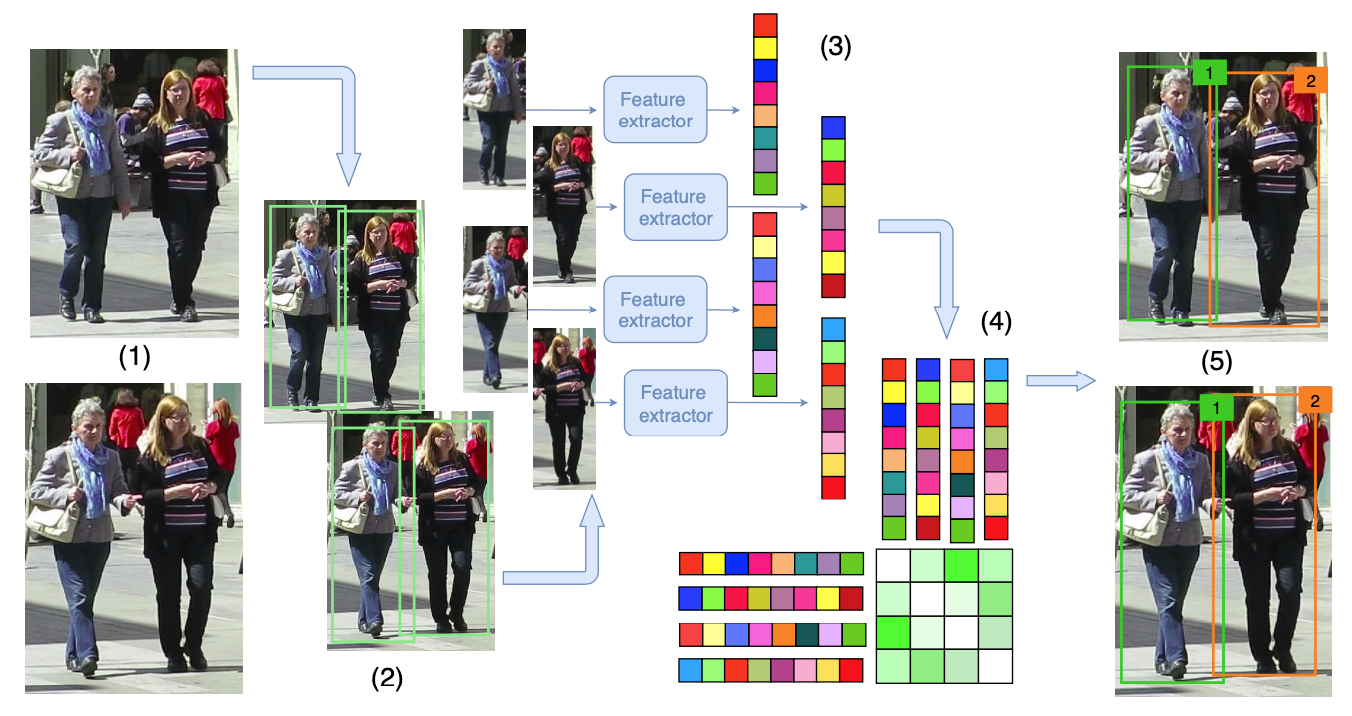
\includegraphics[width=0.9\textwidth]{images/MOT_overview.png}
    \caption{An overview of common MOT algorithms workflow. For each consecutive frames (1), the algorithm first detect all potential objects (2), then extract their representation features (3) and adopt pair-wise comparison (4) to associate most similar objects with the same ID (5). \cite{ciaparrone2020deep}}
    \label{fig:MOT_overview}
\end{figure}
Figure \ref{fig:MOT_overview} shows the step-by-step procedure of common MOT approaches.\\
Common algorithms solved MOT problem can be divided into two main groups: offline and online methods. 
Offline learning (batch based tracking) \cite{rezatofighi2015joint,kim2015multiple} assumes that the system has seen the whole video before start processing. 
Online learning approaches are only allowed to process and update tracking results frame by frame. Due to the efficiency and practicality, online and realtime algorithms achieves more attention. Many works \cite{pang2021quasi, zhou2020tracking, bergmann2019tracking, wojke2017simple} have been proposed to explore this type of learning and achieve potential results on benchmark settings and in practical situations. 
% In the scope of this project, we modified the DeepSORT \cite{wojke2017simple} method as a submodule for our retrieval system.

\subsection{SORT algorithm}
\label{sec:sort}
We first briefly discuss one of the most popular online tracking method, which successfully leverage ConvNet for detection step to achieve state-of-the-art result at the time it proposed, the Simple Online and Realtime Tracking (SORT) \cite{bewley2016simple} algorithm.
The important features of SORT compose: target detections based on Faster-RCNN \cite{NIPS2015_14bfa6bb} architecture, the use of Kalman filter \cite{kalman1960new} to forecast target positions at each time step and Hungarian algorithm \cite{kuhn1955hungarian} for the similarity matching step between current tracks and new detected objects. These modules help to achieve potential accuracy while greatly improves the speed of tracking multiple targets at the same time. \\
\begin{figure}[t!]
    \centering
    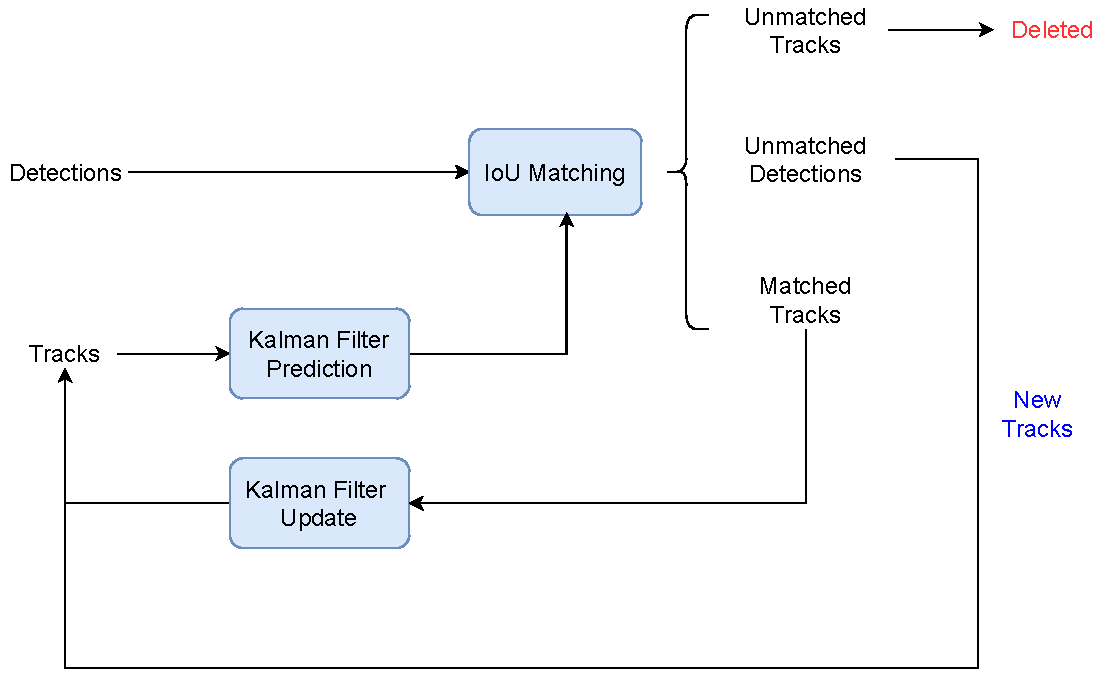
\includegraphics[width=0.9\textwidth]{images/SORT.pdf}
    \caption{SORT algorithm's processing flow.}
    \label{fig:SORT_overview}
\end{figure}
At each time step $t$-th, let $T$ denotes list of tracks we have successfully associate so far, the SORT algorithm works as follow:
\begin{itemize}
    \item \textbf{Detection stage}. \\
    The method utilizes an detector model to detect all potential objects current frame. Suppose that we have $N$ boxes at this frame.
    
    \item \textbf{Kalman Filter prediction stage}. \\
    For each track in $T$, Kalman Filter uses those movement states from previous frames to predicts the target position and speed at current frame. 
    The SORT algorithm works with assumptions that all targets have linear constant velocity and their movements are independent with the others. Hence, a state of target object at a specific time step is implemented as follow.
    \begin{align}
        \label{eqn:sort_kf}
        \mathbf{x} = [u,v,s,r,\dot{u},\dot{v},\dot{s}]
    \end{align}
    where $u, v$ represents the horizontal and vertical coordinate of the target center respectively. While $s$ is the bounding box area and $r$ is the corresponding aspect ratio. $\dot{u},\dot{v},\dot{s}$ denotes the velocity of those values at current time $t$.
    \item \textbf{IOU matching stage}. \\
    Those predicted states at current frame are used to compute a similarity matrix between $T$ tracks and $N$ detected boxes based on IoU score, result in a similar matrix of size $[N \times T]$. Hungary algorithm is then applied on this matrix to produce best matching detection for each track.
    \item \textbf{Confirmation stage}. \\
    Those with similarity score is higher than a threshold are considered as \textit{matched tracks}. Otherwise, tracks with small similarity are seen as disappear from current frame and removed from the system memory. Detections that are not currently matched with any tracks are used to initialize as \textit{new tracks} and saved to the memory.
    \item \textbf{Kalman Filter Update stage}. \\
    The predicted and observed values of matched tracks are linearly weighted to update the current state representation.
\end{itemize}
Figure \ref{fig:SORT_overview} illustrates the workflow of SORT algorithm at each frame.\\
However, SORT algorithm still have some drawbacks when running on those hard cases. The first problem is with the linear assumption of Kalman Filter framework, in practice, the targets rarely move with constant velocity.
And second, ID switches is the biggest drawback of SORT. The association between detections and tracks is simply based on IoU measure, which indicates that the algorithm only cares about the object shape, this causes the phenomenon that the number of ID switches of an object is extremely large when the object is obscured or when the trajectory overlaps with the others.

\subsection{Deep SORT algorithm}
\label{sec:deep_sort}
In this section, we consider another tracking approach that built as an extension to SORT algorithm, Deep SORT \cite{wojke2017simple}. To address the disadvantages of SORT, Deep SORT utilize deep learning network to extract features of detected objects to enhance the data association process. Furthermore, a matching cascade strategy with a new confirmation strategy is proposed to handle the problem of occlusion tracks. These improvements are shown in figure ... .
As compare to figure(SORT), Deep SORT adds a \textit{Matching Cascade} module and a new trajectory confirmation strategy to the original SORT algorithm. \\
To handle the occlusion problem, Deep SORT manages life-cycle of each archived track based on a state variable with three values (\textit{tentative}/\textit{unconfirmed}, \textit{confirmed}, \textit{deleted}). 
\begin{itemize}
    \item Each new track is initialized as \textit{unconfirmed}. Through the filtering process, if the track is not removed in the next three frames, it becomes \textit{confirmed} track, and will stay filtered for the next $max\_age$ frames.
    \item Otherwise, if the track is lost when less then 3 frames are reached, it will be deleted.
\end{itemize}

\begin{figure}[t!]
    \centering
    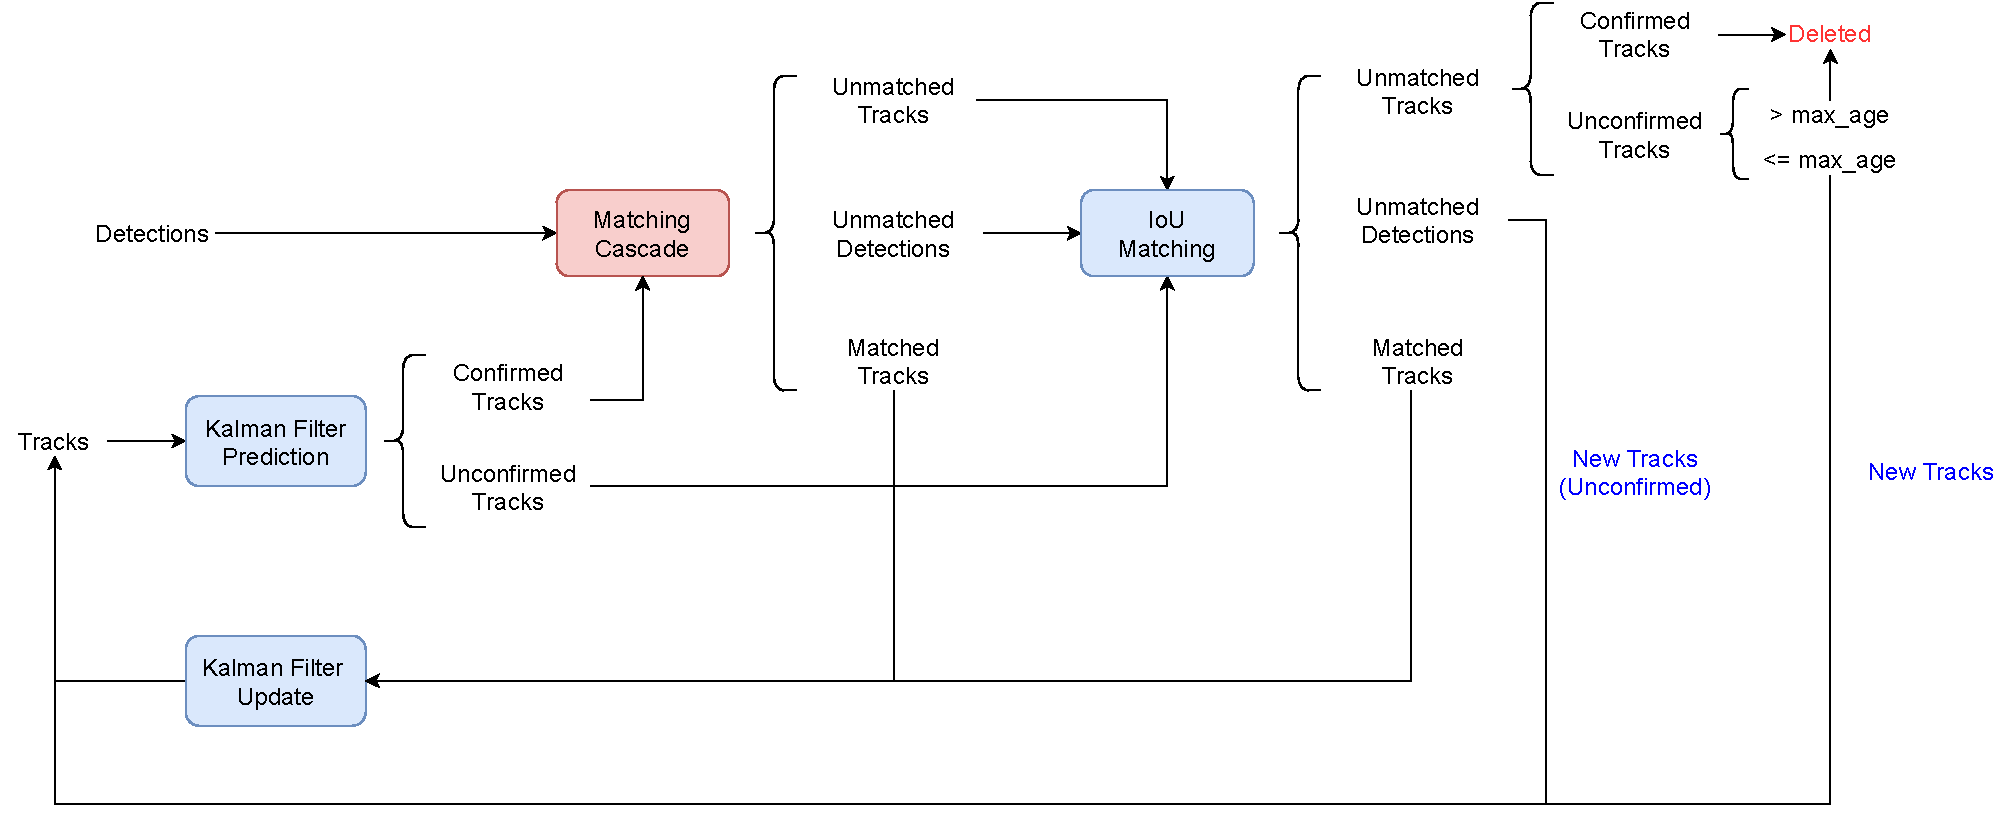
\includegraphics[width=\textwidth]{images/DeepSORT.pdf}
    \caption{Deep SORT algorithm's processing flow.}
    \label{fig:DeepSORT_overview}
\end{figure}

The details of each stage in Deep SORT process are described as follows (shown in figure \ref{fig:DeepSORT_overview}).
\begin{itemize}
    \item \textbf{Detection stage}. \\
    Same as SORT algorithm, Deep SORT use an object detector to detect all potential boxes at current frame.
    \item \textbf{Kalman Fitler Prediction and Update stage}. \\
    Same as SORT algorithm, predict next representation to perform prediction and update current state if finding new detection for each track.
    \item \textbf{Filter Layer 1: Matching Cascade}. \\
    The Matching Cascade takes in a list of archived tracks $T$ and assign them to best matching objects from $N$ detections at current frame. Different from the original SORT, Deep SORT integrates both motion feature and appearance feature to measure the similarity. 
    Motion feature is modelled the same way as the SORT algorithm (\ref{eqn:sort_kf}), while the appearance descriptor is extracted from pretrained CNN-based network trained with re-identification settings. 
    In general, the similarity measure between track $i$ and object $j$ is formulated as follow
    \begin{align}
        \label{eqn:deepsort_score}
        c_{i,j} = \lambda d_{motion}(i, j) + (1-\lambda) d_{appearance}(i, j)
    \end{align}
    Where Mahalanobis distance is used to measure motion uncertainty $d_{motion}$ and Cosine distance is used for appearance measure $d_{appearance}$. \\
    With the computed similarity matrix, Deep SORT then applies multi-step thresholding on archived tracks based on their ages, and finally produce list of matched tracks, unmatched detections and unmatched tracks.
    \item \textbf{Filter Layer 2: IoU Matching}. \\
    This filter apply IoU association with the same strategy as SORT on unlinked tracks and detections from previous layer and archived unconfirmed tracks. 
    \item \textbf{Confirmation stage}. \\
    After the two layers of filtering, unconfirmed tracks that still not match with any detections of confirmed tracks which have stayed too long in the memory (larger than $max\_age$) are removed. Unmatched detections are used to create new tracks and the procedure starts over with the next frame.
\end{itemize}
In the scope of this project, we modified the DeepSORT algorithm \cite{wojke2017simple} to utilize as a sub-module that captures the relationships between target object and neighboring vehicles.

% \section{Semantic Role Labeling}
\label{sec:srl}
Semantic Role Labeling (SRL) task aims to perform semantic analysis of texts that analyzes the propositions expressed by all target verbs of the sentence. 
For each target verb (also known as predicate), all constituents (or arguments) related to that verb are assigned semantic role labels. In common, the task is to extract predicate-argument structure for input sentences to answer the question “who did what to whom, when, where, how and why ?”.
Common solutions for the SRL can be treated as a classification problem performed on each part of the input sentence. 
The methods  aim to classify each part into correct semantic roles with respect to the predicates. \\
Many deep neural networks were proposed to solve the problem with or without detected predicates \cite{zhou2015end, marcheggiani2017simple, he2017deep, tan2018deep, he2018jointly, strubell2018linguistically}. 
The main approach is to apply the sequential models to learn the representations for each input part, then perform classification into a pre-defined set of roles.\\ 
As mentioned in section \ref{sec:BERT}, BERT is a powerful pretraining for such language modeling tasks. Shi, Peng, and Jimmy Lin.\cite{shi2019simple} proposed a BERT-based model to solve the SRL problem and achieve state-of-the-art results on different benchmarks. The method is then applied in various video-text related problems to implement such fine-grained models (discussed in section). 
\begin{figure}[t!]
    \centering
    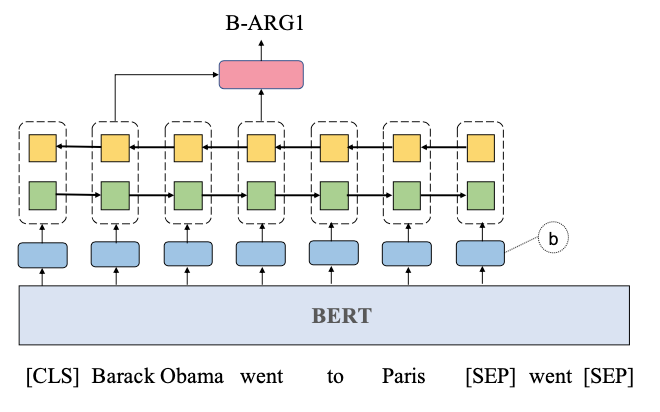
\includegraphics[width=0.7\textwidth]{images/SRL_overview.png}
    \caption{An example of the BERT-based SRL method \cite{shi2019simple} making prediction for the token "Barack".}
    \label{fig:srl_overview}
\end{figure}
The architecture is constructed from BERT encoding followed by a BiLSTM layer, and a one-hidden-layer MLP to produce prediction for each tokens. In more details, the process is as follows (illustrated in figure \ref{fig:srl_overview}):
\begin{itemize}
    \item Given a pair of sentence-predicate $(X, p)$ as input, the input sequence is encoded as [[CLS] sentence [SEP] predicate [SEP]]. This method allows the predicate representation to interact with the whole input context via the self-attention mechanism.
    \item The encoded sequence is then fed into BERT encoder to obtain the sentence representations from [[CLS] sentence [SEP]] tokens. The predicate indicator embedding $\mathbf{b}$ is also associated to locate the predicate positions in the sentence.
    \item The sentence representations are then fed through a BiLSTM layer to get the final representation of each token. 
    \item Finally, to get semantic role prediction for each token, the final hidden state of predicate $\mathbf{h_p}$ is concatenated to that token hidden state $\mathbf{h_i}$ and fed into a feed-forward classifier layer over the pre-defined role set.
\end{itemize}

\textbf{SRL in vision} 
\begin{figure}[!htb]
    \centering
    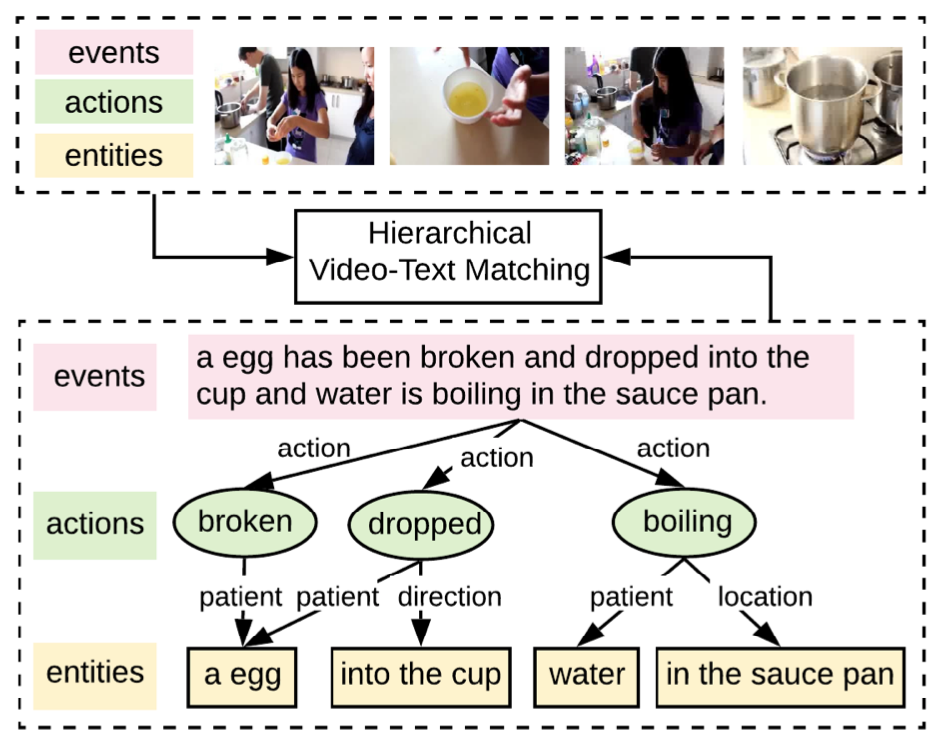
\includegraphics[width=0.7\textwidth]{images/HGR_idea.png}
    \caption{The overview of HGR\cite{chen2020fine} matching process.}
    \label{fig:hgr_overview}
\end{figure}

The SRL task attracts much attention from researchers and has been widely applied in video analytics, where it provides fine-grained cues for matching textual description to correct visual context, such as human object interaction \cite{gupta2015visual}, video question answering \cite{sadhu2021video}, or video grounding \cite{sadhu2020video}, etc. The most related to ours is the utilization of SRL in video-text retrieval. Chen, Shizhe, et al. \cite{chen2020fine} proposed a Hierarchical Graph Reasoning (HGR) model to performs fine-grained retrieval task in many levels (shown in figure \ref{fig:hgr_overview}).
For each input sentence, Shizhe, et al. \cite{chen2020fine} first applies the SRL toolkit \cite{shi2019simple} to obtain predicates and their related semantic role then construct a three-level role graph, including events, actions and entities levels. 
The event node contains the whole input sentence to represent the global context, connected by action nodes that contain the extracted predicates context. The other noun phrases are entity nodes connected to different action nodes. The directed edges between action nodes and entity nodes indicate their semantic role relation.\\
In our work, the input query describes different attributes of the target objects, we apply SRL toolkit\cite{shi2019simple} to extract these signals to perform refinement and re-ranking to enhance the retrieval results.




\section{Segmentation}
\label{sec:segmentation}
Segmentation is one of the most important tasks in image processing and has a long history of development. It has grown strongly since neural networks and computing resources starting to explode. One of the basic ideas behind segmentation is that you can use convolution layers as a feature extraction mechanism. By downsampling the input image after passing it through a backbone CNN model containing multiple pooling layers, you can generate a prediction at a smaller scale that needs to be upsampled to the original image size. This approach, which uses fully convolutional layers to perform classification for each pixel in the feature map, is known as Fully Convolutional Networks (FCNs)\cite{FCN}.

The reason behind this architecture that combine deep semantic information in deeper layers and spatial information in shallow layers together. However, there are still many limitations, such as losing spatial information in the downsampling process; its inability to leverage global context information; and the lack of a mechanism for variant-scales.

The next popular method is using encoder and decoder based architecture. Segnet\cite{segnet} is the pioneer when do a symmetric architecture between encoder and decoder. In details, decoder mirror copy of the decoder and augment with information from encoder. There are multi descendants inspire from this and popular nowadays like Unet\cite{Unet}

Unet\cite{Unet} is one of the most popular architectures in computer vision, and it has been shown to be very effective in medical applications. The encoder provides spatial information that helps to decode the features more accurately. There are variants of Unet that have been developed specifically for better performance, such as Unet++\cite{UnetPP} and Attention U-Net\cite{AttUnet}. These variants continue to show promise for semantic segmentation tasks, with improved accuracy over other methods.

Another model to approach the fixed kernel size problem is of the family of segmentation models called DeepLab\cite{Deeplab}. DeepLab model family is a promising solution to the fixed kernel size problem. They use dilated convolution (also known as atrous convolution) to learn features from a larger region without increasing computational expenses. This allows for deeper neural networks, which can better capture complex patterns in data. Atrous Convolutions with different rates are stacked in the encoder, called the Atrous Spatial Pyramid Pooling module. This module offers the ability to learn multi-scale features in the encoding phase, which is important for accurately capturing information about objects and scenes.

Computer vision has come a long way in the past few years. Researchers have found that transformer power is one of the potential ways to improve computer vision. Transformers are famous for their ability in downstream task in natural language processing. However, the naive usage that replaces transformer vision as a feature extraction is not exploiting almost its capability. Due to that TransUnet\cite{TransUnet} use the strong point of them ideas, which is transformer leverage both detailed high-resolution spatial information from CNN features and the global context encoded by Transformers, also inspired by the u-shaped architectural design 

\section{Uncertainty Estimation}
\label{sec:uncertainty}

Data is growing bigger everyday, but that is still not enough for deep neural networks. The empirical report of \cite{mahajan2018exploring}, \cite{joulin2016learningvisual} suggests that the performance of recent deep networks is not yet saturated with respect to the size of training data, since data are mostly unlabeled. For this reason, learning methods from semi-supervised learning to unsupervised learning are attracting attention of many researchers. However, given a fixed amount of data, performance of semi-supervised or unsupervised still cannot match with that of fully-supervised learning. 
Thus, the data annotation has a vital part in uplifting the performance of neural networks
Having said that, what then is the suitable approach while the budget for annotation is limited?  \cite{atlas1989trainingconnectionist} first proposed active learning where a model actively selects data points that the model is uncertain of. The core idea of active learning is that the most informative data point would be more beneficial to model improvement than a randomly chosen data point.

Active learning has been advancing in the recent decades. Given a scenario where a labeled dataset \mathcal{L} and an unlabeled dataset \mathcal{U} is available, active learning aims to select a fixed number of subset of samples from \mathcal{U} to be labeled such that they can lead to improvement in model performance. To identify the most valuable examples to be labeled, many sampling strategies have been proposed in previous research, and it is mostly the main focus of those. Data points chosen by these strategies are expected to be able assist model to become more generalized and comprehensive after training.

Given a pool of unlabeled data, there have been two major approaches according to the selection criteria: uncertainty-based, diversity-based and expected model change

Uncertainty-based strategy [\cite{joshi2009multi}, \cite{wang2016cost}, \cite{tong2001svmactive}, \cite{seung1992query}, \cite{beluch2018power}] selects samples for which the model produces most uncertain predictions while the diversity approach [\cite{sener2018activelearningforcnn}, \cite{nguyen2004activepreclustering}, \cite{guo2010activeinstance}] selects diverse data points that can represent the entire distribution of the unlabeled pool.
Expected model change [\cite{roy2001toward}, \cite{settles2007multiple}, \cite{freytag2014selecting}] selects data points that brings great impact to the training model parameters or its outputs.

The most straightforward method of the uncertainty approach is to utilize class posterior probabilities to define uncertainty. Despite its simplicity, this approach has performed remarkably well in various tasks, such as object detection \cite{wang2018towardshuman}, semantic segmentation \cite{jain2016activesegmentationprop} and human pose estimation \cite{liu2017activehumanpose}.

Recently, Gal et al. \cite{gal2017deep} obtains uncertainty estimation from deep networks through multiple forward passes by Monte Carlo Dropout \cite{gal2016dropout}. It was shown to be effective for classification with small datasets, but according to [32], it does not scale to larger datasets.

Interestingly, \cite{yoo2019learningloss} train an additional regression module, which uses the training loss as optimization target, to predict a score for each unlabeled sample to evaluate its worthiness for labeling. 

The majority of empirical results from previous researches suggest that active learning is actually reducing the annotation cost. The problem is that most of methods require task-specific design or are not efficient in the recent deep networks.

\begin{figure}[h]
    \centering
    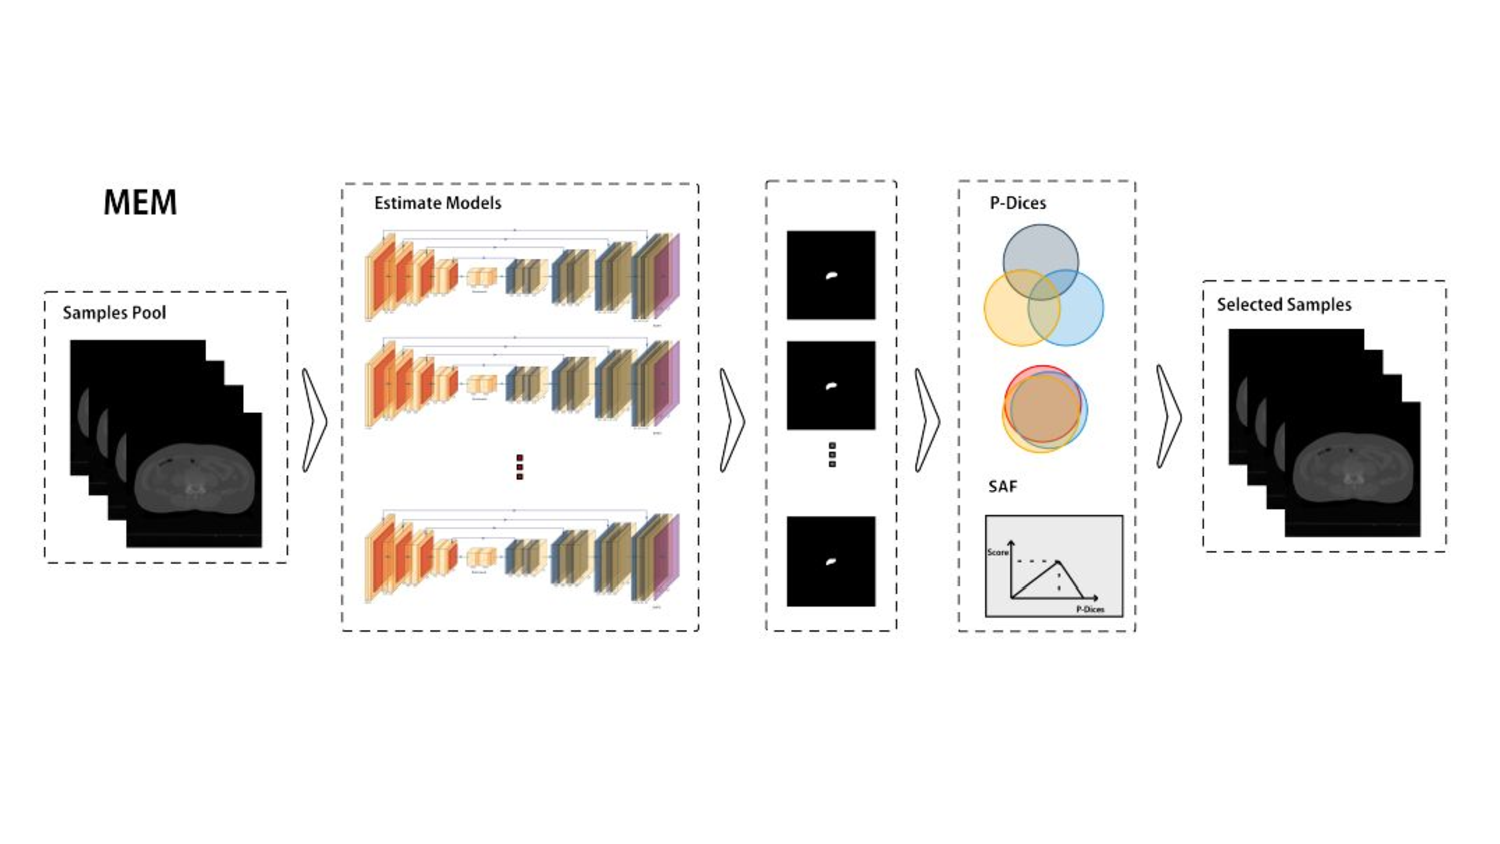
\includegraphics[width=\textwidth]{content/resources/new_images/related_works/pdices.pdf}
    \caption{A pipeline for active learning proposed in \cite{wang2019twostagequery}, which calculate unlabeled sample score through the two-step query strategy: P-Dices and SAF}
    \label{fig:pdices}
\end{figure}

As a task-agnostic uncertainty approach, \cite{seung1992query}, \cite{beluch2018power} train multiple models to construct a committee, and measure the consensus between the multiple predictions from the committee. \cite{wang2019twostagequery} goes with the same strategy where the authors compute the entropy between numerous trained agents, as depicted in Figure \ref{fig:pdices}.

We follow \cite{wang2019twostagequery} to use deep ensemble to generate prediction for each unlabeled sample, then based on consensus entropy to select good samples. While previous works aim at finding the most uncertain samples to be manually labeled by experts, but in our context, manual annotation is forbidden, therefore we try to find most certain samples that can be used for retraining.
\section{Semi-supervised learning}
\label{sec:semisup}

With the constantly increasing volume of non-annotated raw data in practice, semi-supervised learning approaches have been gaining popularity in the area of deep learning recently to effectively utilize this source of data.  
Recent works focus on two of the most common semi-supervised methods, which are consistency regularization and pseudo-labeling.

Consistency regularization aims at enforcing the consistency between the predictions (or intermediate features) of two different views of an unlabeled input sample. 
Some prior works \cite{kim2020structuredloss}, \cite{french2019semi} add perturbation to the input sample, then forward both the original and perturbed one through the same network to generate two augmented outputs. These two outputs are forced to be similar by the regularization function. This approach can be seen as attaching an unsupervised branch to the supervised learning paradigm.

On the other hand, pseudo-labeling, a.k.a., self-learning, self-labeling, or decision-directed learning, is initially developed for using unlabeled data in classification. Recently, it is applied for semi-supervised segmentation \[\cite{zheng2021rectifying}, \cite{chen2020naivestudent}, \cite{zhu2020improving}, \cite{zoph2020rethinking} \], . Frequently, it involves more than one model to produce pseudo-labels by converting model predictions on unlabeled samples into soft or hard labels as optimization targets for retraining. The process can be iterated several times. Various schemes are introduced on how to decide the pseudo segmentation maps. For example, the GAN-based methods [\cite{hung2018adversarial}, \cite{mittal2019semi}, \cite{souly2017semisupervised}], use the discriminator learned for distinguishing the predictions and the ground-truth segmentation to select high-confident segmentation predictions on unlabeled images as pseudo segmentation.

One common type of approach is teacher-student settings. The teacher, which usually is the larger network, is fully-supervisedly trained on the labeled data while generating pseudo-labels on unlabeled data to guide the student model to learn more stably \[\cite{tarvainen2017meanteachers}, \cite{cui2019semisupervised}, \cite{hang2020localnglobal}, \cite{wang2020double}, \cite{yu2019uncertainty}\]. Often, The teacher's parameters are updated using an exponential moving average from the student's parameters \cite{cui2019semisupervised}. 

Apart from the teacher-student paradigm, many proposals are the variance of it. As discussed in \cite{ke2019dualstudent}, because of exponential moving average, teacher network in mean-teacher tends to be very close to the student when the training process converges.

Dual-student [\cite{hang2020localnglobal}, \cite{ke2020guided}, \cite{cao2022adversarial}], for instance, is proposed to use two independently initialized student network without teacher and has been achieving great performance as well. One examplar is \cite{chen2021semisupervised}, which has been adopted in our work, trains 2 segmentation models simultaneously on both labeled and unlabeled data. Basically, with two source images as input, they generate a cutmix version by combining them as one image and mixing the two pseudo segmentation maps obtained from the models. Afterward, the mixed pair of image and mask is used as supervision of the two segmentation networks. 
Developed from that, \cite{luo2021semisupervised} incorporates the idea that those two models should have different architectures to boost the performance by far, one of them should be conventional CNNs while the other has a transformers-based structure. 

Recently, SSL has been widely used for medical image computing to reduce the
annotation efforts [\cite{hang2020localnglobal}, \cite{li2020transformation}, \cite{ma2020active}, \cite{peng2020mutual}]. Bai et al \cite{bai2017semisupervised} developed an iterative framework where in each iteration, pseudo labels for unannotated images are predicted by the network
and refined by a Conditional Random Field (CRF) then the new pseudo labels are used
to update the network. 

We desire to build the same framework as \cite{bai2017semisupervised} in which multiple models, in which choosen architectures are inspired from \cite{luo2021semisupervised}, are used to refine the pseudo labels. 

However, one inherent weakness of the pseudo label learning is that the pseudo label usually contains noisy predictions. Despite the fact that most pseudo labels are correct, wrong labels also exist, which could compromise the subsequent training. If the model is fine-tuned on the noisy label, the error would also be transferred to the
adapted model. Therefore, we also integrate active learning to decide which pseudo labels are suitable for retraining the	 model.
\section{Mask Propagation}
\label{sec:mask_propagate}

Video object segmentation is a task that requires specific objects to be segmented in a given video. In terms of Semi-supervised settings, a first-frame annotation is provided by the user, and the method segments objects in all remaining frames automatically. This technique, which uses a mask as prior knowledge to predict other masks, is called Mask Propagation.

To propagate these sparse labels through the entire video sequence, traditional methods often solve an optimization problem with an energy defined over a graph structure \cite{badrinarayanan2010label}, \cite{vijayanarasimhan2012active}, \cite{avinash2014seamseg}.

Early deep neural network methods rely on fine-tuning the networks at test time to make segmentation networks focus on target objects and then inference on all other frames, which are extremely slow. Among them, OSVOS \cite{caelles2017one} and MoNet \cite{xiao2018monet} finetune pre-trained networks on the first-frame ground-truth at test time. OnAVOS \cite{voigtlaender2017online} extends the first-frame fine-tuning by introducing an online adaptation mechanism. Following these approaches, MaskTrack \cite{perazzi2017learning} and PReM \cite{luiten2018premvos} utilize optical flow to help propagate the segmentation mask from one frame to the next. Despite achieving promising results, the test-time fine-tuning restricts networks’ efficiency. 
Faster approaches have been proposed such as temporal CNN, capsule routing \cite{duarte2019capsulevos}, tracking, space-time matching, and memory-based methods:

\textbf{Temporal CNN}. Recurrent methods propagate information often from the most recent frames, either via a mask \cite{perazzi2017learning} or via a hidden representation \cite{ventura2019rvos}, \cite{hu2017maskrnn}. These methods are prone to drifting and struggle with occlusions.

\textbf{Tracking}
In contrast, tracking-based approaches \cite{jang2017online}, \cite{wang2019fast}, \cite{chen2020state} perform
frame-to-frame propagation and are thus efficient at test-time. They however lack long-term context and often lose track after object occlusions.

\textbf{Space-time matching}. While some methods \cite{huang2020fast}, \cite{voigtlaender2019feelvos} \cite{yang2020collaborative} also include the first reference frame for global matching, the context is still limited and it becomes harder to match as the video progresses

\textbf{Memory-based}. To address the context limitation, recent state-of-the-art methods use more past frames as feature memory \cite{oh2019stm}, \cite{duarte2019capsulevos}, \cite{huang2020fast} ,\cite{ge2021video}, \cite{cheng2021stcn}, \cite{cheng2022xmem}, \cite{yang2022associating}. These approaches leverage a memory network to embed past-frame predictions into memory and apply non-local attention mechanisms to propagate object information from the memory to the current frame. Our work strongly adopts the memory-based style. 

Oh et. al \cite{oh2019stm} introduces a framework which extract embeddings from multiple intermediate frames and store inside the memory. Then in forwarding stage, these memories are combined with the query embeddings to segment the object

\begin{figure}[!h]
    \centering
    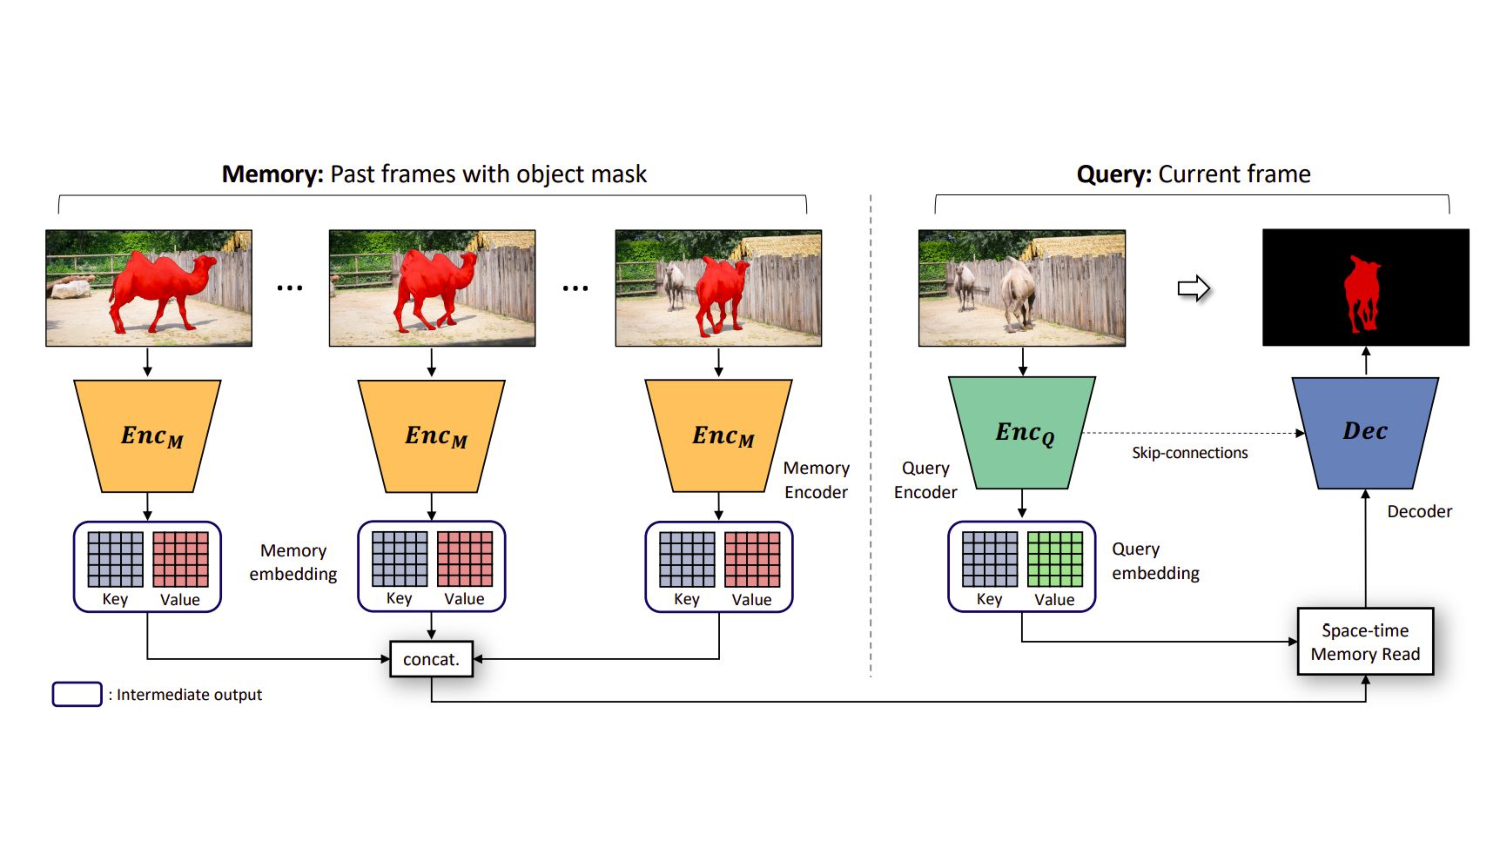
\includegraphics[width=\textwidth]{content/resources/new_images/models/stm.pdf}
    \caption{Overview architecture of STM \cite{oh2019stm}.}
    \label{fig:stm}
\end{figure}

Cheng et. al  \cite{cheng2021mivos} proposes a framework in which the user initially scribbles a mask of an object, the scribble is transformed into the real binary mask (S2M), then that mask is propagated through every video frame based on STM \cite{oh2019stm}. Then the user can choose some incorrect frames and scribble to guide the fusion with the propagated frame to output more accurate masks (Different-aware fusion).

\begin{figure}[!h]
    \centering
    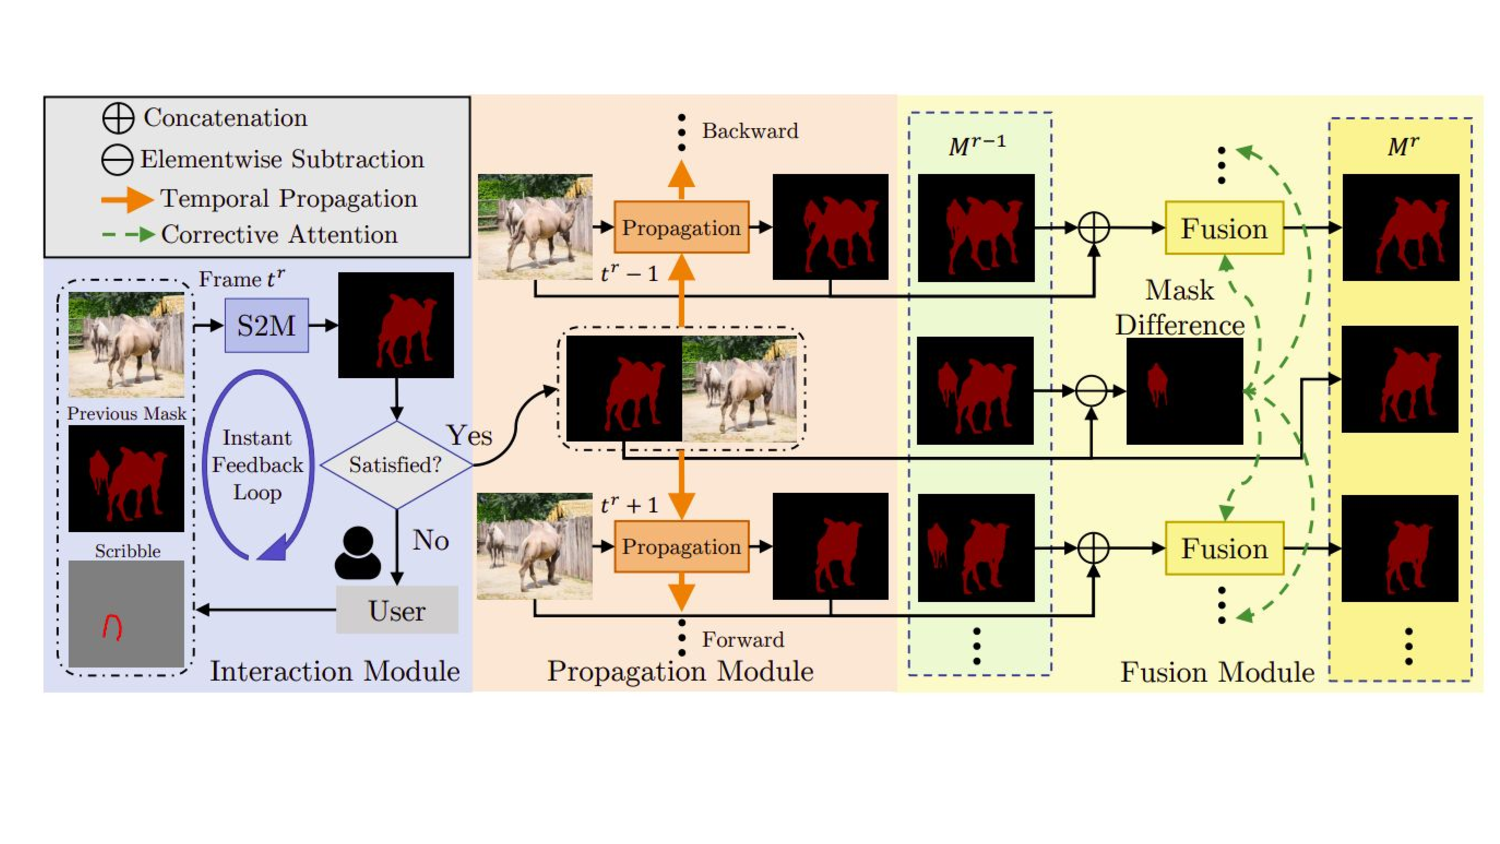
\includegraphics[width=\textwidth]{content/resources/new_images/models/mivos.pdf}
    \caption{Overview architecture of MiVOS \cite{cheng2021mivos}}
    \label{fig:mivos}
\end{figure}

Among these extensions, we adapt STCN \cite{cheng2021stcn} as one of our main modules for refinement as it is simple and effective. but with minor modification. However, most variants cannot handle long videos due to the ever-expanding feature memory bank of STM.

\begin{figure}[!h]
    \centering
    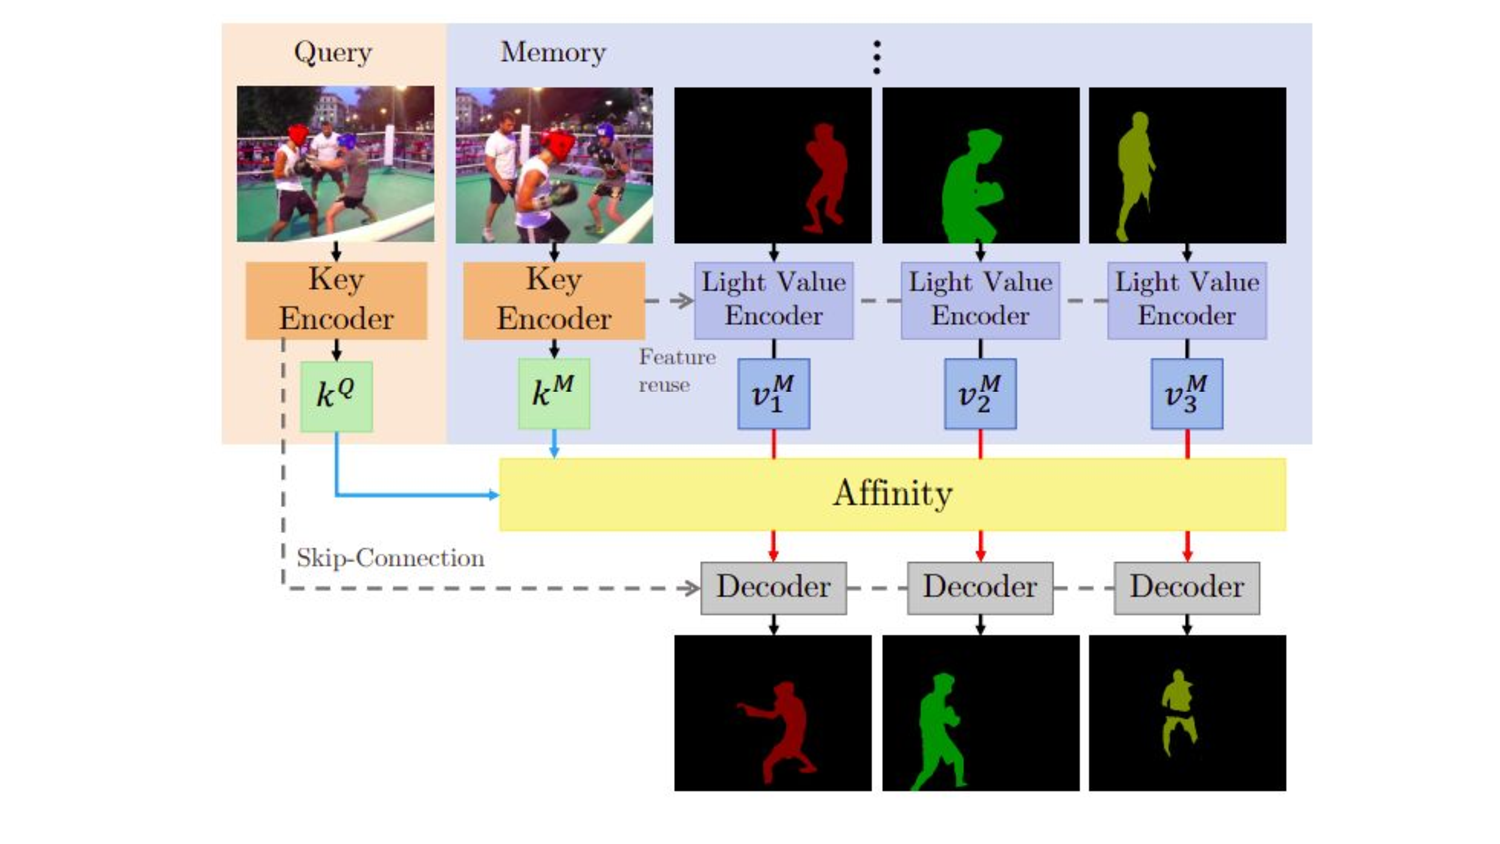
\includegraphics[width=\textwidth]{content/resources/new_images/models/stcn.pdf}
    \caption{Overview architecture of STCN \cite{cheng2021stcn}}
    \label{fig:stcn}
\end{figure}

Nonetheless, the mask propagation and segmentation are still computed individually for different objects. The
problem restricts the application and development of the VOS with multiple targets. Hence,  \cite{yang2022associating} proposes AOT to associate and decode multiple targets simultaneously, as efficiently as processing a single object. Moreover, it is the first method to utilize Transformer modules inside mask-propagation

\begin{figure}[!h]
    \centering
    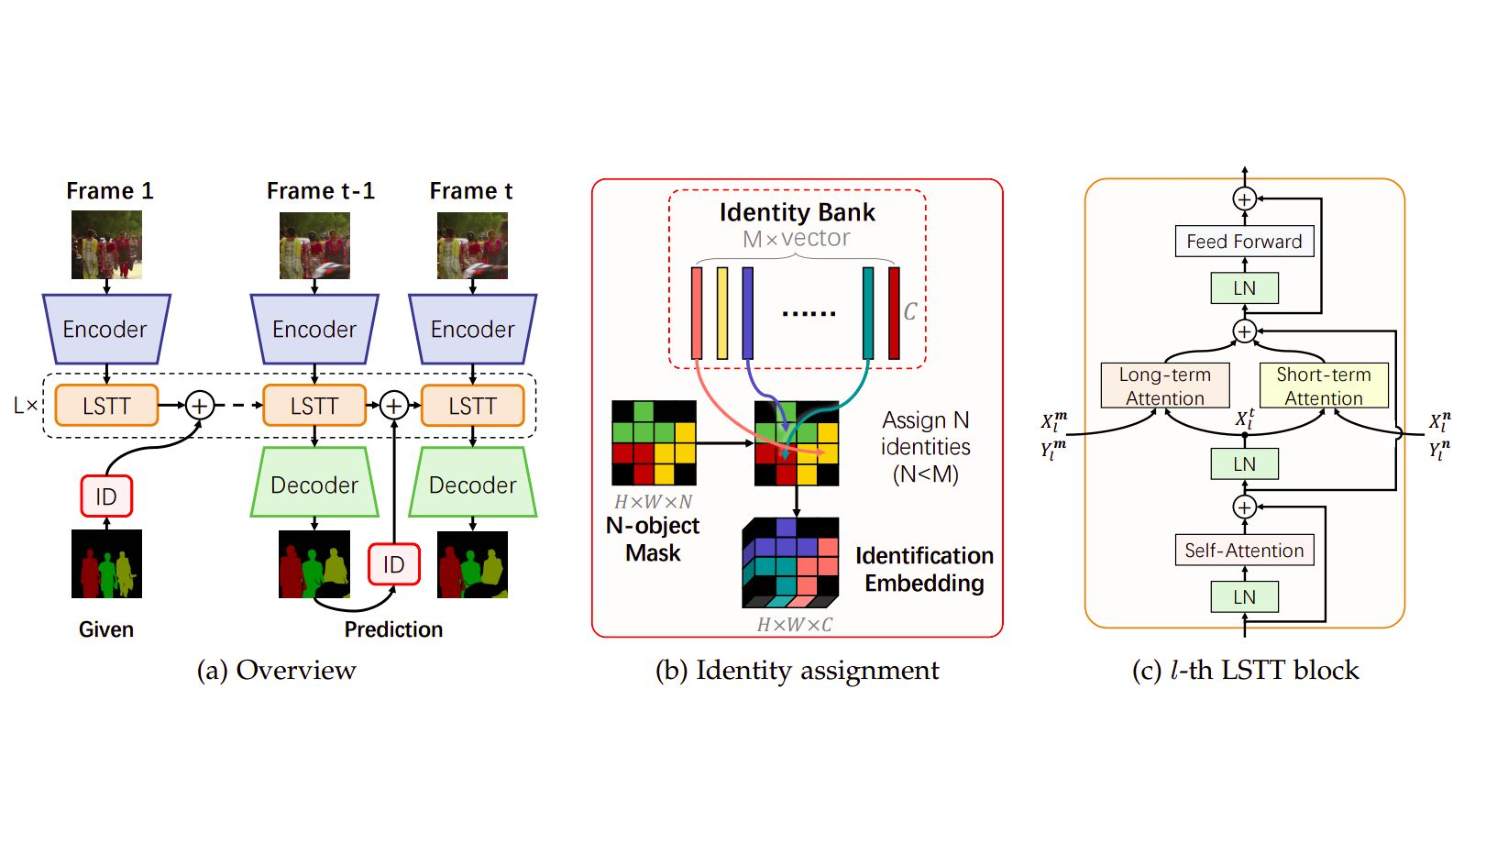
\includegraphics[width=\textwidth]{content/resources/new_images/models/aot.pdf}
    \caption{Overview architecture of AOT \cite{yang2022associating}}
    \label{fig:aot}
\end{figure}

Yet, it still does not solve the GPU memory explosion problem. Recently, authors of STCN \cite{cheng2021stcn}, develop XMem \cite{cheng2022xmem} which uses multiple memory stores to capture different temporal contexts while keeping the GPU memory     usage strictly bounded due to the long-term memory and consolidation.

\begin{figure}[!h]
    \centering
    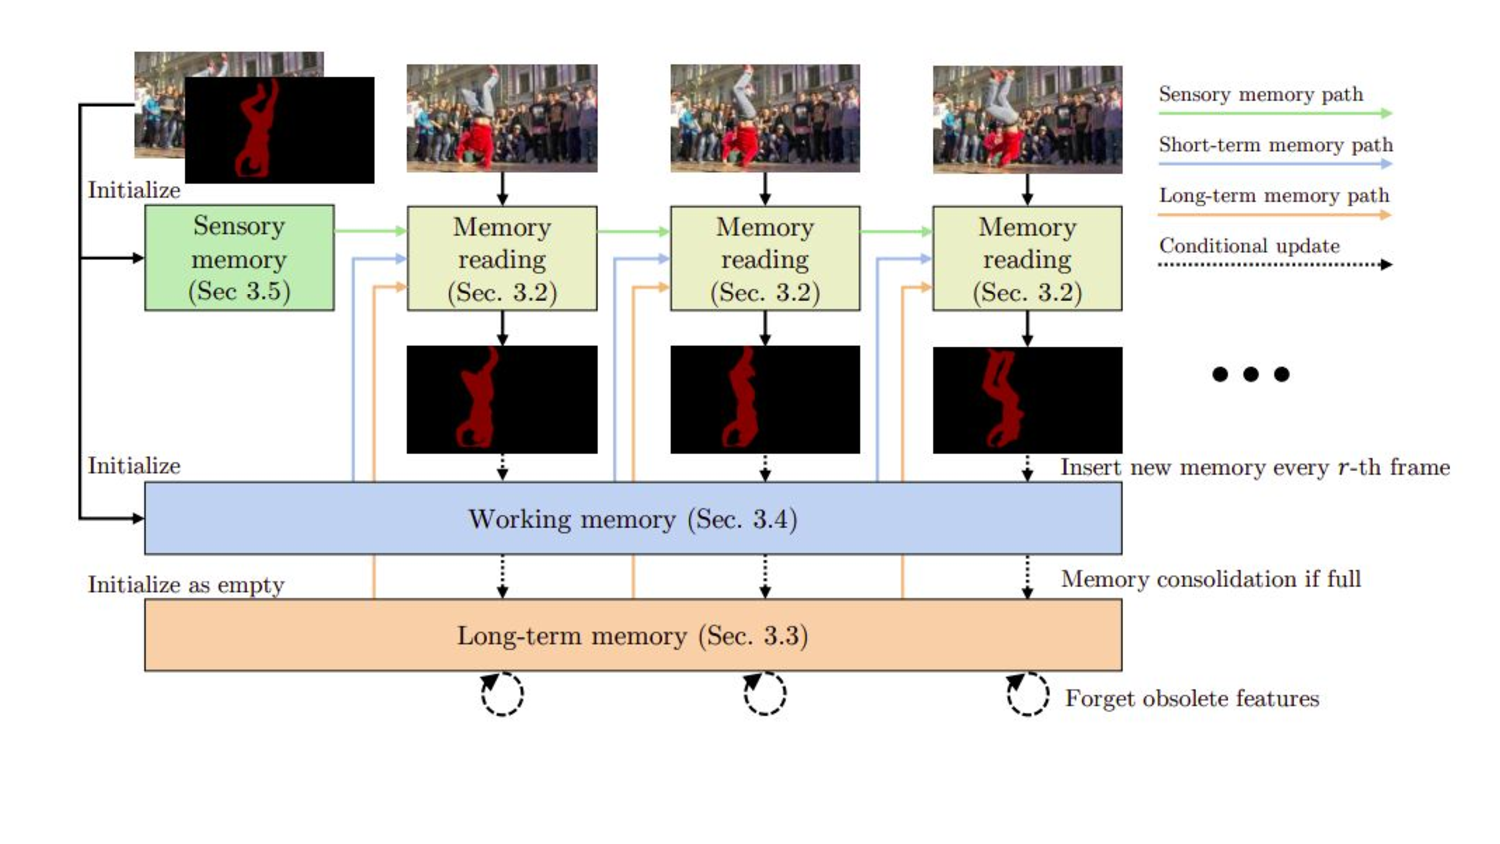
\includegraphics[width=\textwidth]{content/resources/new_images/models/xmem.pdf}
    \caption{Overview architecture of XMem \cite{cheng2022xmem}}
    \label{fig:xmem}
\end{figure}


Although video object segmentation has yielded promising results in a number of domains, these approaches have not been exploited for medical dataset creation. The use of medical images for training and testing machine learning algorithms is critical to the development of accurate models that can be used to diagnose and treat diseases. In order to improve the accuracy and effectiveness of machine learning algorithms for medical image analysis, it is important to develop novel methods specifically tailored for this domain. Mask propagation is a popular technique in interactive scenarios of video object segmentation. 

The user will refine the inputs to the algorithm in order to segment the target objects more accurately. Our proposed concept is heavily inspired by the DAVIS Challenge on Video Object Segmentation. After the first raw prediction of the associate model, the user will interact with some of the valuable slices. After that, they will submit their predicted masks to a server for review. In each of these subsequent interactions, from a list of slices specified by themselves, they choose one frame with an uncertain prediction and provide it to a server who then provides them with a new set of scribbles in this frame which points out regions that are false positives or negatives 




\section{Temporal Position Encoding}
\label{sec:positional_encoding}

After the breakthrough of deep learning in still-image recognition originated with the introduction of the AlexNet model \cite{krizhevsky2012imagenet}, there has been active research devoted to the design of deep networks for a sequence of images. 

Many attempts in the past leverage CNNs trained on images to extract features from the individual frames and then perform temporal integration of such features into a fixed-size descriptor using pooling, high-dimensional feature encoding, or recurrent neural networks. Karpathy et al. \cite{karpathy2014large} presented a thorough study on how to fuse temporal information in CNNs and proposed a “slow fusion” model that extends the connectivity of all convolutional layers in time and computes activations through temporal convolutions in addition to spatial convolutions. Time-series models have also been widely studied in this task to exploit the capabilities of long-term memory features, like LSTM \cite{hochreiter1997long} or GRU \cite{cho2014properties} or most recently, Transformer \cite{vaswani2017attention}. 

However, different from RNN and LSTM, the self-attention inside Transformer cannot capture position information by design. This is critical, considering that the model is otherwise entirely invariant to the sequence order, which is harmful to video encoding.

One common approach is to use position encodings which are combined with input elements to
expose position information to the model. These position encodings can be a deterministic function of position (\cite{sukhbaatar2015end}; \cite{vaswani2017attention}) or learned representations. 
Convolutional neural networks inherently capture relative positions within the kernel size of each convolution. They have been shown to still benefit from position encodings (\cite{gehring2017convolutional}), however.
For the Transformer, which employs neither convolution nor recurrence, incorporating explicit
representations of position information is an especially important consideration since the model is
otherwise entirely invariant to sequence order.

To overcome this issue, \cite{jung2020global} adopts relative position embedding \cite{shaw2018self}, which ensures translation-equivariance property and allows the model to generalize unseen sequence length during training. Empirically, \cite{jung2020global}  confirms that relative position indeed helps to capture the sequential properties of video content, improving the video encoder' performance further.

In our work, we implement a simple way to inject the position information into the feature vector for the model to learn, in the hope that the target model will be capable of understanding relatively the location of specific objects within a long sequence, in our case a CT volume.

In fact, looking at the problem of abdomen organ segmentation in CT volume, this position embedding can be seen as a model constraint since any organ of a human only appear in certain areas. Therefore, with the introduction of this information, the model can comprehend the knowledge of organ relative position to make a better prediction. 

Many previous works manipulate model outputs by incorporating conditions to the model inputs or intermediate features. \cite{mirza2014cgan} first introduce encoding label information into both discriminator and generator to control the generation of the image. \cite{messina2021transformer} also has its own way to concatenate encoded bounding-boxes values to the input vector for the model to learn. All these mentioned research uses only simple embedding layers to embed the scalar values, which encourages us to do the same. 